%%%%%%%%%%%%%%%%%%%%%%%%%%%%%%%%%%%%%%%%%
% Twenty Seconds Resume/CV
% LaTeX Template
% Version 1.0 (14/7/16)
%
% This template has been downloaded from:
% http://www.LaTeXTemplates.com
%
% Original author:
% Carmine Spagnuolo (cspagnuolo@unisa.it) with major modifications by 
% Vel (vel@LaTeXTemplates.com) and Harsh Gadgil
%
% License:
% The MIT License (see included LICENSE file)
%
%%%%%%%%%%%%%%%%%%%%%%%%%%%%%%%%%%%%%%%%%

%----------------------------------------------------------------------------------------
%    PACKAGES AND OTHER DOCUMENT CONFIGURATIONS
%----------------------------------------------------------------------------------------

\def\zh_CN_CV{1}

%\documentclass[letterpaper]{twentysecondcv} % a4paper for A4
\documentclass[utf8]{twentysecondcv} % a4paper for A4
%\usepackage[utf8]{inputenc}

% Command for printing skill progress bars
\newcommand\skills{ 
~
    \smartdiagram[bubble diagram]{
        \textbf{Self-motivated}\\\textbf{Dev},
        \textbf{Relational/}\\\textbf{Document}\\\textbf{DB},
        %\textbf{~~~~OOP~~~~~},        
        \textbf{Latex/}\\\textbf{Markdown},
        \textbf{Web}\\\textbf{Stuff},
        \textbf{Machine}\\\textbf{Learning},
        \textbf{Deep}\\\textbf{Learning},
        \textbf{Hardware}\\\textbf{Programming},
        \textbf{Computer}\\\textbf{Vision}
    }
}

%\interests{{Functional Programming/4.5},{ML DL/5},{Software Engineering/6},{Computer Vision/6}}
% Programming skill bars
\programming{{Java $\textbullet$ JS $\textbullet$ HTML / 3.5}, {C++ $\textbullet$ C  $\textbullet$ Arduino / 4.5},  {OpenCV $\textbullet$ Python $\textbullet$ Markdown / 6}}


% Projects text
\experience{
\textbf{TJU RM 成员} \\ 算法组成员,基于视觉、深度学习方法的物体检测与跟踪 \\
        \textbf{研究生助教} \\ 大一新生程序设计实践 I 助教,教授为外籍老师,课程全英文教学 \\
        \textbf{Python 101} \\ 为几位已申请到国外高校的金融专业准硕士/博士准备的 python 课程 \\
        \textbf{志愿者教师} \\ “滴水行动”,与队友一起在陕西省铜川市一山村小学志愿教学,活动由陕西青年与环境互助网络组织进行
        %\textbf{Club activities} - Member of Young Volunteer team and Work-study centre clubs in Xidian.
}


%----------------------------------------------------------------------------------------
%     PERSONAL INFORMATION
%----------------------------------------------------------------------------------------

% If you don't need one or more of the below, just remove the content leaving the command, e.g. \cvnumberphone{}



\cvname{{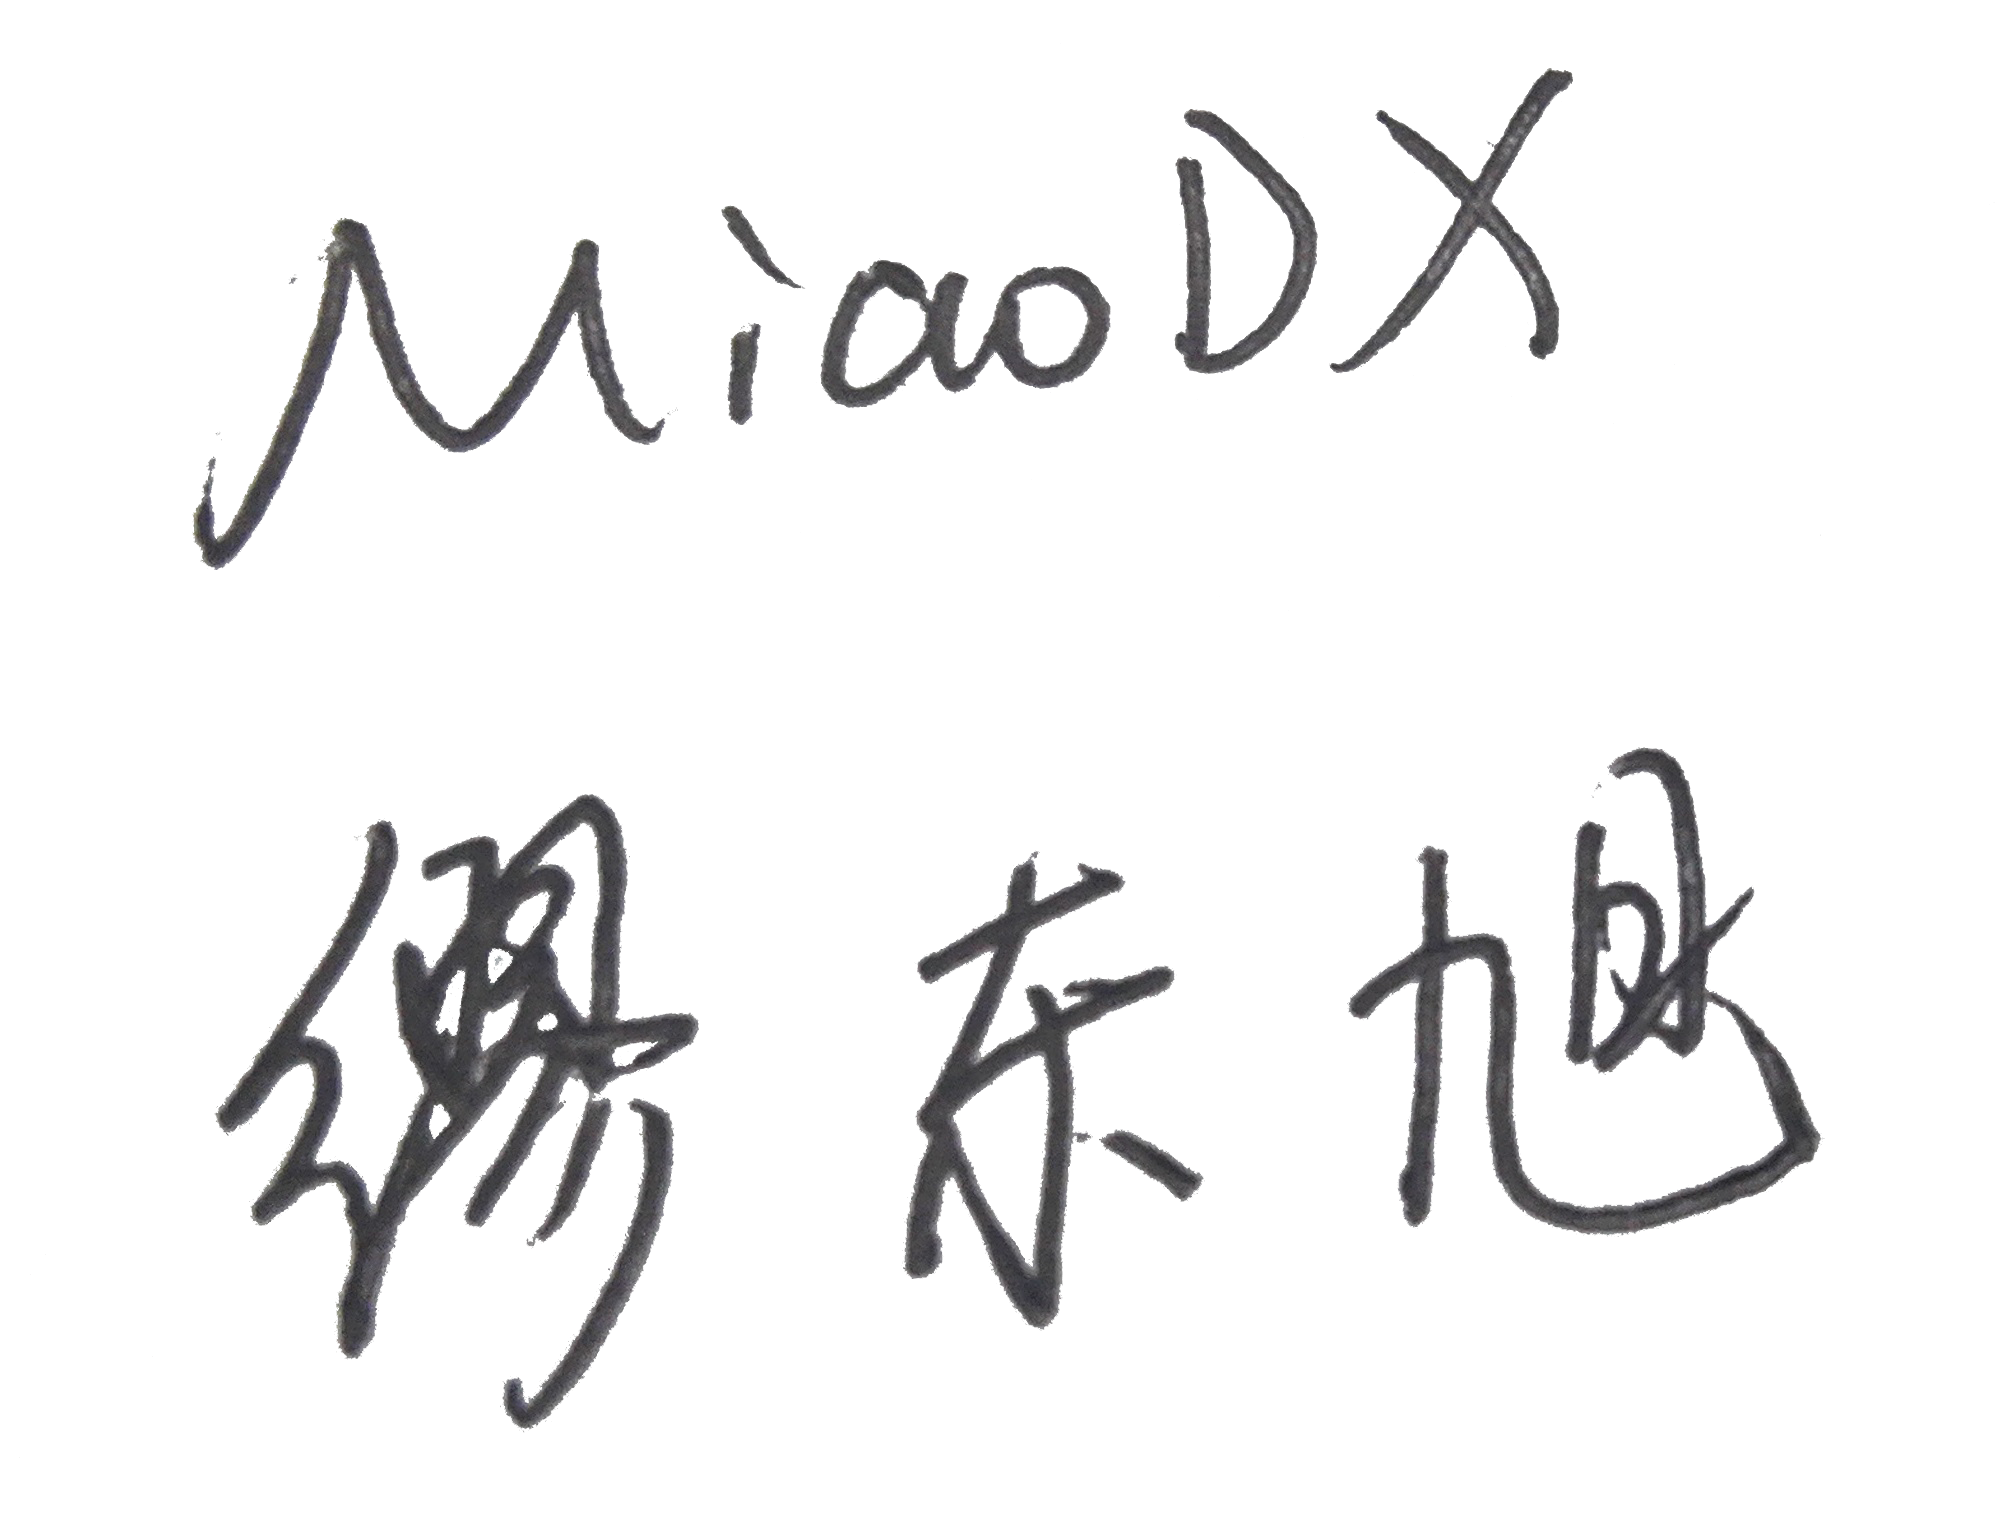
\includegraphics[scale=0.04]{img/miaodx_name.png}}} % Your name
\cvjobtitle{ Graduate Student, \\ Self-motivated Developer} % Job title/career

%\cvlinkedin{https://linkedin.com/in/miaodx}
\cvgithub{https://github.com/MiaoDX}
\cvnumberphone{+86 13502009660} % Phone number
\cvsite{https://miaodx.github.io/} % Personal website
\cvmail{miaodx@tju.edu.cn} % Email address

%----------------------------------------------------------------------------------------

\begin{document}

\makeprofile % Print the sidebar

%----------------------------------------------------------------------------------------
%     EDUCATION
%----------------------------------------------------------------------------------------
\section{教育背景}

\begin{twentyshort}
    \twentyitemshort
        {2016 - Now}
        {硕士\ 软件工程\ \ 计算机视觉,机器人 \hfill{天津大学}}	
	\twentyitemshort
		{2012 - 2016}
		{学士\ 软件工程 \hfill{西安电子科技大学}}		
\end{twentyshort}




\section{会议文章}

\begin{twenty}
    \twentyitem
        {Jan 2018}
        {}        
        {ICASSP 2018, CCF-B 类会议接收 (第一作者)}
        {}
        {}
        {ACTIVE CAMERA RELOCALIZATION WITH RGBD CAMERA
FROM A SINGLE 2D IMAGE}
    \twentyitem
        {Mar 2018}
        {}        
        {ICME 2018, CCF-B 类会议接收 (Oral)}
        {}
        {}
        {Fast and Reliable Computational Rephotography on Mobile Device}
\end{twenty}

\section{项目经验}
\begin{twenty}

    \twentyitem
        {}
        {}        
        {列举部分近期项目,更多的请访问 github 主页}
        {\href{https://github.com/MiaoDX/}{github.com/MiaoDX}}
        {}
        {}
    
        
    \twentyitem
    {July 2018 - }
    {Sep. 2018}
    {地平线机器人 (Horizon Robotics) 实习}
    {}
    {}
    {自动驾驶研发部门感知算法工程师实习生,工作内容涉及深度学习、标注工具、交通流建模以及基于消失点的车道线检测等。}
          
    \twentyitem
    {Jan 2018 - }
    {May 2018}
    {ICRA 2018 DJI ROBOMASTER 人工智能挑战赛}
    {}
    {}
    {搭建全自动智能车与大疆官方的 AI 智能车进行对抗。主要负责视觉算法,物体识别、跟踪及部分决策模块。(Finalist invitation)}
    
    \twentyitem
    {Mar 2016 -}
    {Present}
    {主动相机位姿重定位}
    {}
    {}
	{主动地将相机位姿重定位到参考位置是机器人学与计算机视觉一基础研究领域,支撑了本科毕设与会议论文。}
    %{Actively relocate camera to previous pose is one fundamental research area in robotics and computer vision. Major part of my undergraduate graduation and conference papers.}
    
	\twentyitem
        {Python}
		{Data Label}
        {机器学习/深度学习\ 数据标注工具}
        {\href{https://github.com/MiaoDX/DataLabel}{DataLabel}}
        {}
        {物体检测数据标注工具,利用跟踪算法大幅减少手工标注的需求量,可用于输出 Dlib 与 Darkflow 适用的物体检测训练配置文件。}
          
    \twentyitem
        {Virtual Env}
      	{DL}
        {UnrealCV 与深度学习结合 (Faster-RCNN)}
        {\href{https://github.com/MiaoDX/unrealcv_examples/}{UnrealCV \& DL}}
        {}
        {将 \href{https://github.com/smallcorgi/Faster-RCNN\_TF}{smallcorgi/Faster-RCNN\_TF} 集成到 \href{https://github.com/unrealcv/unrealcv}{UnrealCV} 上,探究通过虚拟环境生成的合成数据来提升现有深度学习实现的可能性。}
                 
    \twentyitem
        {Python}
		{RL}
        {增强学习应用到吃豆人游戏}
        {\href{https://github.com/MiaoDX/hand_in_homework/tree/master/Advanced\_AI/}{PacMan \& RL}}
        {}
        {整理了增强学习的一些基础知识,并将其应用到吃豆人游戏当中,在高级人工智能结课比赛中取得较好成绩。}
        
		\twentyitem
        {OpenCV}
        {Flask}
        {Restful 深度相机}
        {\href{https://github.com/MiaoDX/depth\_camera}{Depth\_camera \& http}}
        {}
        {将一双目深度相机(ZED)扩展成为 Restful 服务,能被不同编程语言调用,省去了为每种语言进行 SDK 移植的麻烦。}

	    \twentyitem
        {Python}
		{ML}
        {利用 sklearn 库处理 UCI Adult 数据集}
        {\href{https://github.com/MiaoDX/scikit\_learning/}{scikit\_learning}}
        {}
		{基于人口调查结果,使用 sklearn 机器学习库来预测收入是否超过 \$50K/yr,这是一典型的分类问题,达到 85\%+ 的精度。}
		
        \twentyitem
        {Java}
       	{BP}
        {使用 Java 实现反向传播算法}
        {\href{https://github.com/MiaoDX/bp_java}{BP\_java}}
        {}                
        {在使用流行的开源 ML(\/DL) 库前,能够先从头实现一些基本的组件是很重要的,可以对其理论基础与运算机理有更深的了解。}
		
		\twentyitem
        {Node.js}
        {MongoDB}
        {考勤管理系统}
        {\href{https://github.com/SEAPC2016/attendance}{Attendance system}}
        {}
        {为一(模拟)公司实现基于 RESTful 接口的考勤管理系统。公司成员可以经由系统申请休假并等待批准,同时可以查询由系统整理得到的历史统计数据。}

\end{twenty}

\section{荣誉奖励}

\begin{twentyshort}
    \twentyitemshort
        {2018-2019}
        {华为奖学金,校级一等奖学金}
    \twentyitemshort
        {2017-2018}
        {校级二等奖学金}
	\twentyitemshort
        {2016-2017}
        {校级一等奖学金}
	\twentyitemshort
		{Oct 2016}        
		{研究生推免至天津大学软件学院}
	\twentyitemshort
		{2014-2015}
		{国家励志奖学金}
	\twentyitemshort
		{2014CUMCM}
		{全国大学生数学建模竞赛,陕西赛区二等奖}
	\twentyitemshort
		{2013-2014}
		{校级二等奖学金}		
	\twentyitemshort
		{2012-2013}
		{校级一等奖学金}		
\end{twentyshort}        


\section{其他信息}


\begin{twentyshort}
    \twentyitemshort
        {Passed CET-6, English as working language}
        {}
	\twentyitemshort
        {阅读\ 跑步\ 拳击\ 骑行}
        {}
\end{twentyshort}        

\end{document} 
